\documentclass[12pt, a4paper]{article}


\usepackage{wrapfig}
\usepackage{graphicx}
\usepackage[T1]{fontenc}
\usepackage[polish]{babel}
\usepackage[utf8]{inputenc}
\usepackage[font=footnotesize, labelfont=bf]{caption}
\usepackage{csquotes}
\usepackage{placeins}
\usepackage{booktabs}
\usepackage{siunitx}


\usepackage[backend=biber, sorting=ynt]{biblatex}
\addbibresource{draft.bib}

\newcommand{\code}[1]{\texttt{#1}}


\title{Bibliography
management:
\texttt{biblatex}
package}


\author{Krzytsztof
Wiśniewski}
\date{
}


\begin{document}
  \begin{titlepage}
    \centering


    \Large \textbf{UNIWERSYTET GDAŃSKI}\\ \textbf{WYDZIAŁ MATEMATYKI, FIZYKI I
    INFORMATYKI}

    \vspace{2.5cm}


    \large \textbf{Krzysztof Wiśniewski}\\ \textbf{numer albumu: 274276}

    \vspace{1.5cm}
    \raggedright \small Kierunek studiów: Bioinformatyka\\ Specjalność: Ogólna

    \vspace{1.5cm}


    \centering
    \Large \textbf{Optymalizacja oprogramowania w języku Python do analizy stanów kwantowych.}

    \vfill


    \raggedleft \normalsize Praca licencjacka\\ wykonana\\ pod kierunkiem\\ dr hab.
    Marcin Wieśniak, prof. UG\\

    \vfill


    \centering
    \large Gdańsk 2023
  \end{titlepage}
  \newpage


  \tableofcontents
  \newpage


  \begin{sloppypar}
    \begin{abstract}
      W tej pracy przeprowadzam analizę efektywności metod optymalizacji, która
      koncentruje się na minimalizacji czasu wykonania, oprogramowania napisanego w języku
      Python\cite{Python_Language}\cite{ML_Learning_Python}, skupiającego się na
      arytmetyce macierzowej, na przypadku programu CSSFinder służącego do analizy stanów
      kwantowych pod kątem detekcji splątania kwantowego. Pośród rozważanych metod
      obecna będzie standardowa implementacja w języku Python z wykorzystaniem
      biblioteki NumPy\cite{NumPy_Article}\cite{NumPy_Doc}, wersja wzbogacona o kompilację
      JIT przy pomocy biblioteki Numba\cite{Numba_Article}\cite{Numba_Doc}, wersja
      skompilowana do kodu maszynowego przy pomocy biblioteki Cython\cite{Cython_The_Best_Of_Both}\cite{Cython_Org}
      i kompilatora GCC\cite{GCC_Org} oraz implementacja w języku Rust\cite{Rust_Programming_Language},
      również skompilowana do kodu maszynowego.
    \end{abstract}

    \section{Wstęp}


    \subsection{Dlaczego Python?}


    Język Python zachęca użytkowników prostotą składni, łatwością tworzenia kodu,
    dynamicznym systemem typów, automatycznym zarządzanie pamięcią, mnogością dostępnych
    bibliotek otwartoźródłowych, oraz rozbudowaną społecznością programistów. Na
    przestrzeni ostatnich 20 lat język stworzony przez Guido van Rossum zanotował
    intensywny wzrost popularności. Pokazują to liczne zestawienia, w tym zestawienie
    najczęściej wykorzystywanych języków programowanie na GitHub'ie\cite{GitHub_Top_languages},
    w którym Python w roku 2022 zajął 2 miejsce, czy też zestawienie TIOBE Index\cite{TIOBE_Software_Index},
    uznające ten język za obecnie najbardziej rozpowszechniony pośród doświadczonych programistów
    (Maj 2023).

    \FloatBarrier
    \begin{figure}[h]
      \centering
      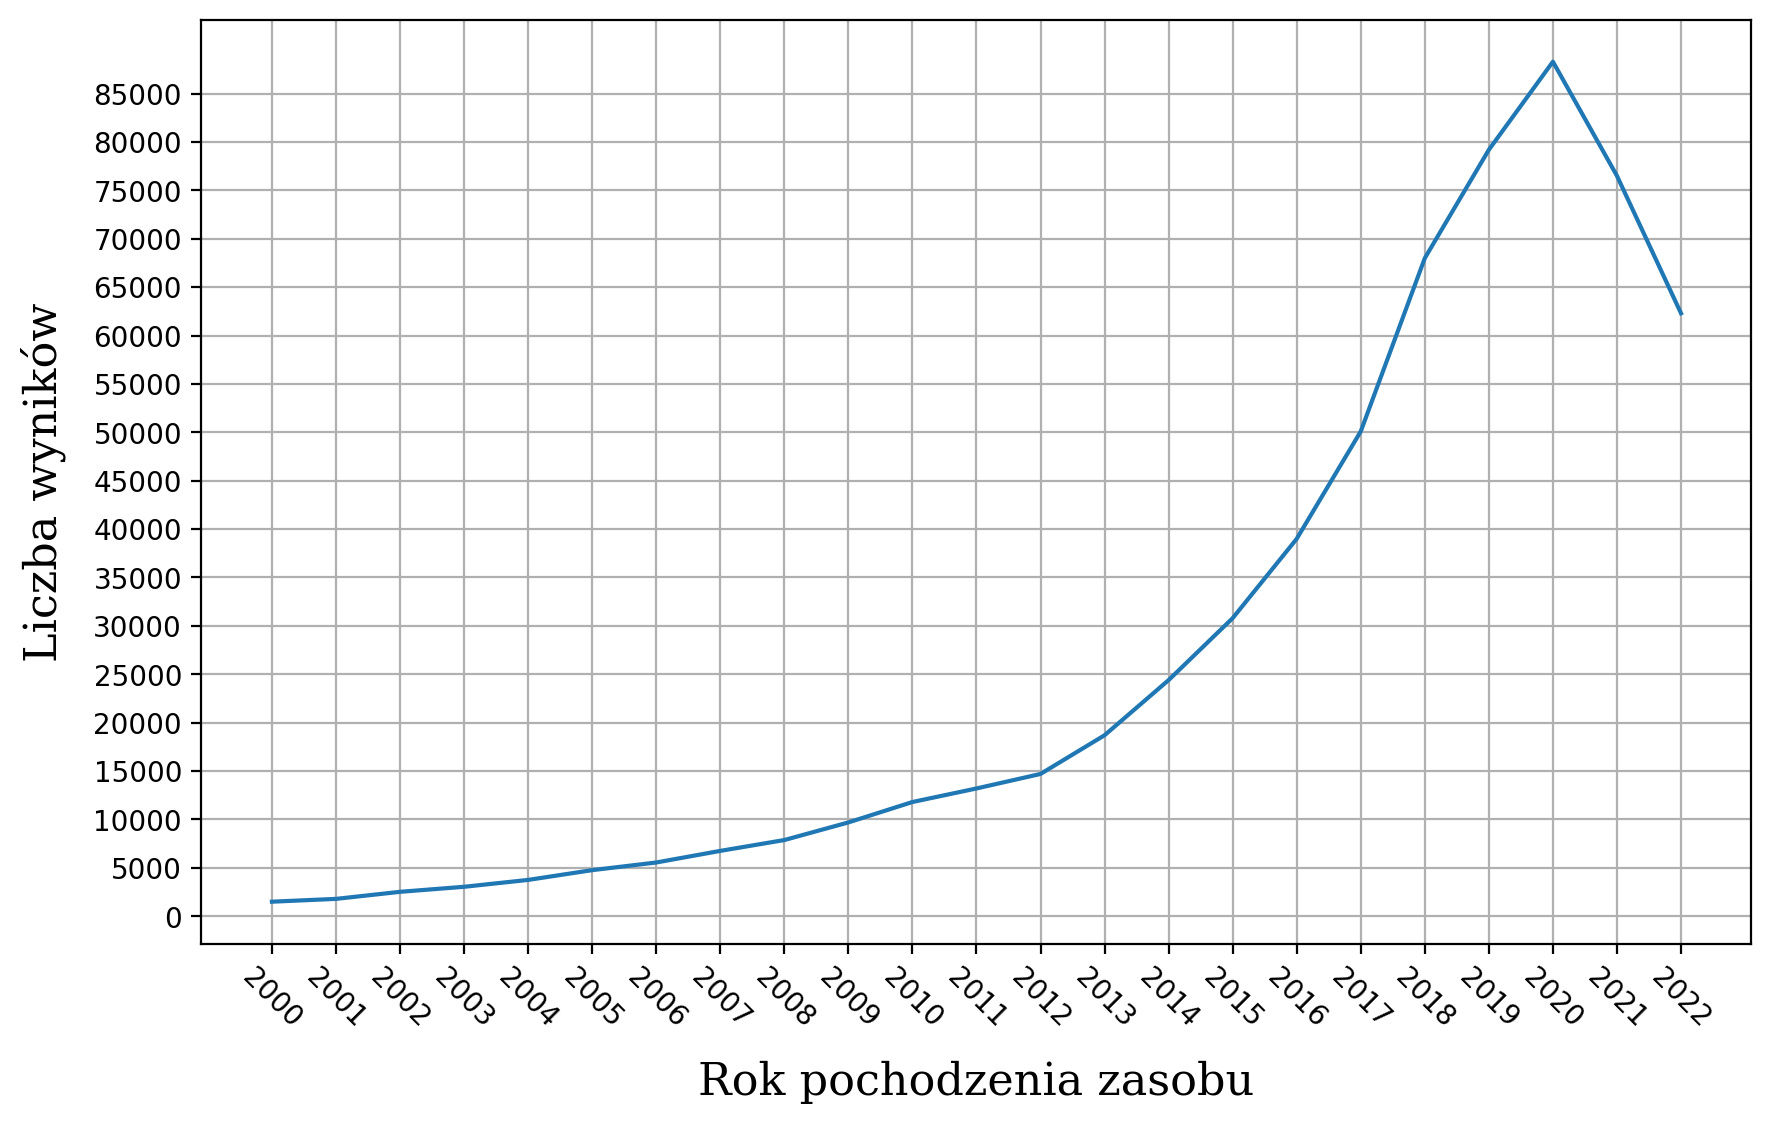
\includegraphics
      [width=0.75\textwidth]{"resources/images/python_language_results.png"}
      \caption{Ilość wyników zwróconych przez wyszukiwarkę Google Scholar dla zapytania 'python language' z podziałem na rok wydania.}
    \end{figure}
    \FloatBarrier

    Niestety, interpretowany kod, napisany w Pythonie, pomimo licznych zalet, posiada
    również dotkliwą wadę - pod względem wydajności znacząco odstaje od kompilowanych
    języków programowania (C\cite{C_vs_Python}, C++\cite{Cpp_vs_Python}, Rust\cite{Rust_vs_Python}).
    Natomiast, dzięki nakładowi pracy wielu zespołów programistów, obecnie istnieją
    metody pozwalające na obejście tej niedogodności.

    \subsection{Cel pracy}


    Praca ta ma na celu weryfikację efektywności wybranych metod poprawy czasu wykonania
    oprogramowania CSSFinder, zaimplementowanego w języku Python. W dalszej jej części
    opiszę specyfikę poszczególnych metod optymalizacji, w jaki sposób zmieniają wydajność
    programu oraz spróbuję wskazać prawdopodobne powody dla których niektóre z uzyskanych
    wyników konsekwentnie odstają od oczekiwań które można mieć wobec wykorzystanych narzędzi.

    Do przeprowadzenia takich analiz konieczne było wielokrotne ponowne implementowanie algorytmu.
    Funkcjonalny kod opisywany w tej pracy dostępny jest w repozytoriach Gita\cite{Git_Com}
    w serwisie GitHub \cite{CSSFinder_New}\cite{CSSFinder_New_Numpy}\cite{CSSFinder_New_Rust}.
    W skutek prac projektowych utworzona została również grupa publicznych pakietów, które
    można pobrać z serwisu PyPI:
    \begin{itemize}
      \item \code{cssfinder}\cite{CSSFinder_New_PyPI}

      \item \code{cssfinder\_backend\_numpy}\cite{CSSFinder_New_Numpy_PyPI}

      \item \code{cssfinder\_backend\_rust}\cite{CSSFinder_New_Rust_PyPI}
    \end{itemize}
    Zainstalowanie ich jest możliwe przy pomocy menadżera pakietów języka Python\cite{Packaging_PEPs},
    np. \code{pip}\cite{PIP}. Pakiety są kompatybilne z implementacją CPython w wersjach
    3.8 - 3.10 i były testowane na systemach Windows (10), Linux (Ubuntu 22.04) oraz macOS
    (12).

    \subsection{Pochodzenie programu}


    Program CSSFinder bazuje na algorytmie zaproponowanym przez E. Gilberta\cite{Lindemann_Gilbert}
    pozwalającym na znalezienie odległości pomiędzy punktem, a zbiorem wypukłym. Korzysta
    z faktu że możliwe jest zastosowanie tego algorytmu do analizy stanów kwantowych pod
    kątem detekcji splątania kwantowego\cite{MW_Hilbert_Schmidt_distance}\cite{MW_Gilbert_Quantum_Entanglement}.
    Algorytm ten wielokrotnie, z sukcesem, był wykorzystany do analizy problemów z
    dziedziny fizyki kwantowej\cite{MW_56_Year_Algorithm}\cite{MW_Variational_approach}.

    \section{Metody}


    \subsection{Wstępne profilowanie}


    Prace nad optymalizacją kodu rozpocząłem od wstępnego profilowania pracy programu w
    trybie 1 (full separability of an n-quDit state) na układzie 5 qubitów (macierz $32\times
    32$ podwójnej precyzji zmiennoprzecinkowych liczb zespolonych) do uzyskania 1000
    korekcji. Wykorzystałem do tego moduł z biblioteki standardowej języka Python, \code{cProfile}.
    Ze względu na silnie obciążającą procesor naturę programu i stosunkowo krótki czas
    pracy, istniała obawa że dodatkowe obciążenie ze strony modułu \code{profile}
    mogłoby zafałszować wyniki, dlatego preferowane było wykorzystanie \code{cProfile}. Przy
    analizie tak uzyskanych wyników posiłkowałem się wizualizacjami wykonanymi przy pomocy
    biblioteki \code{snakeviz}\cite{Snakeviz_PyPI}. Podczas testów, program wykorzystywał
    domyślny globalny generator biblioteki NumPy (PCG64\cite{NumpyDefaultGenerator}) z
    ziarnem ustawionym na wartość 0.

    \FloatBarrier
    \begin{figure}[h]
      \centering
      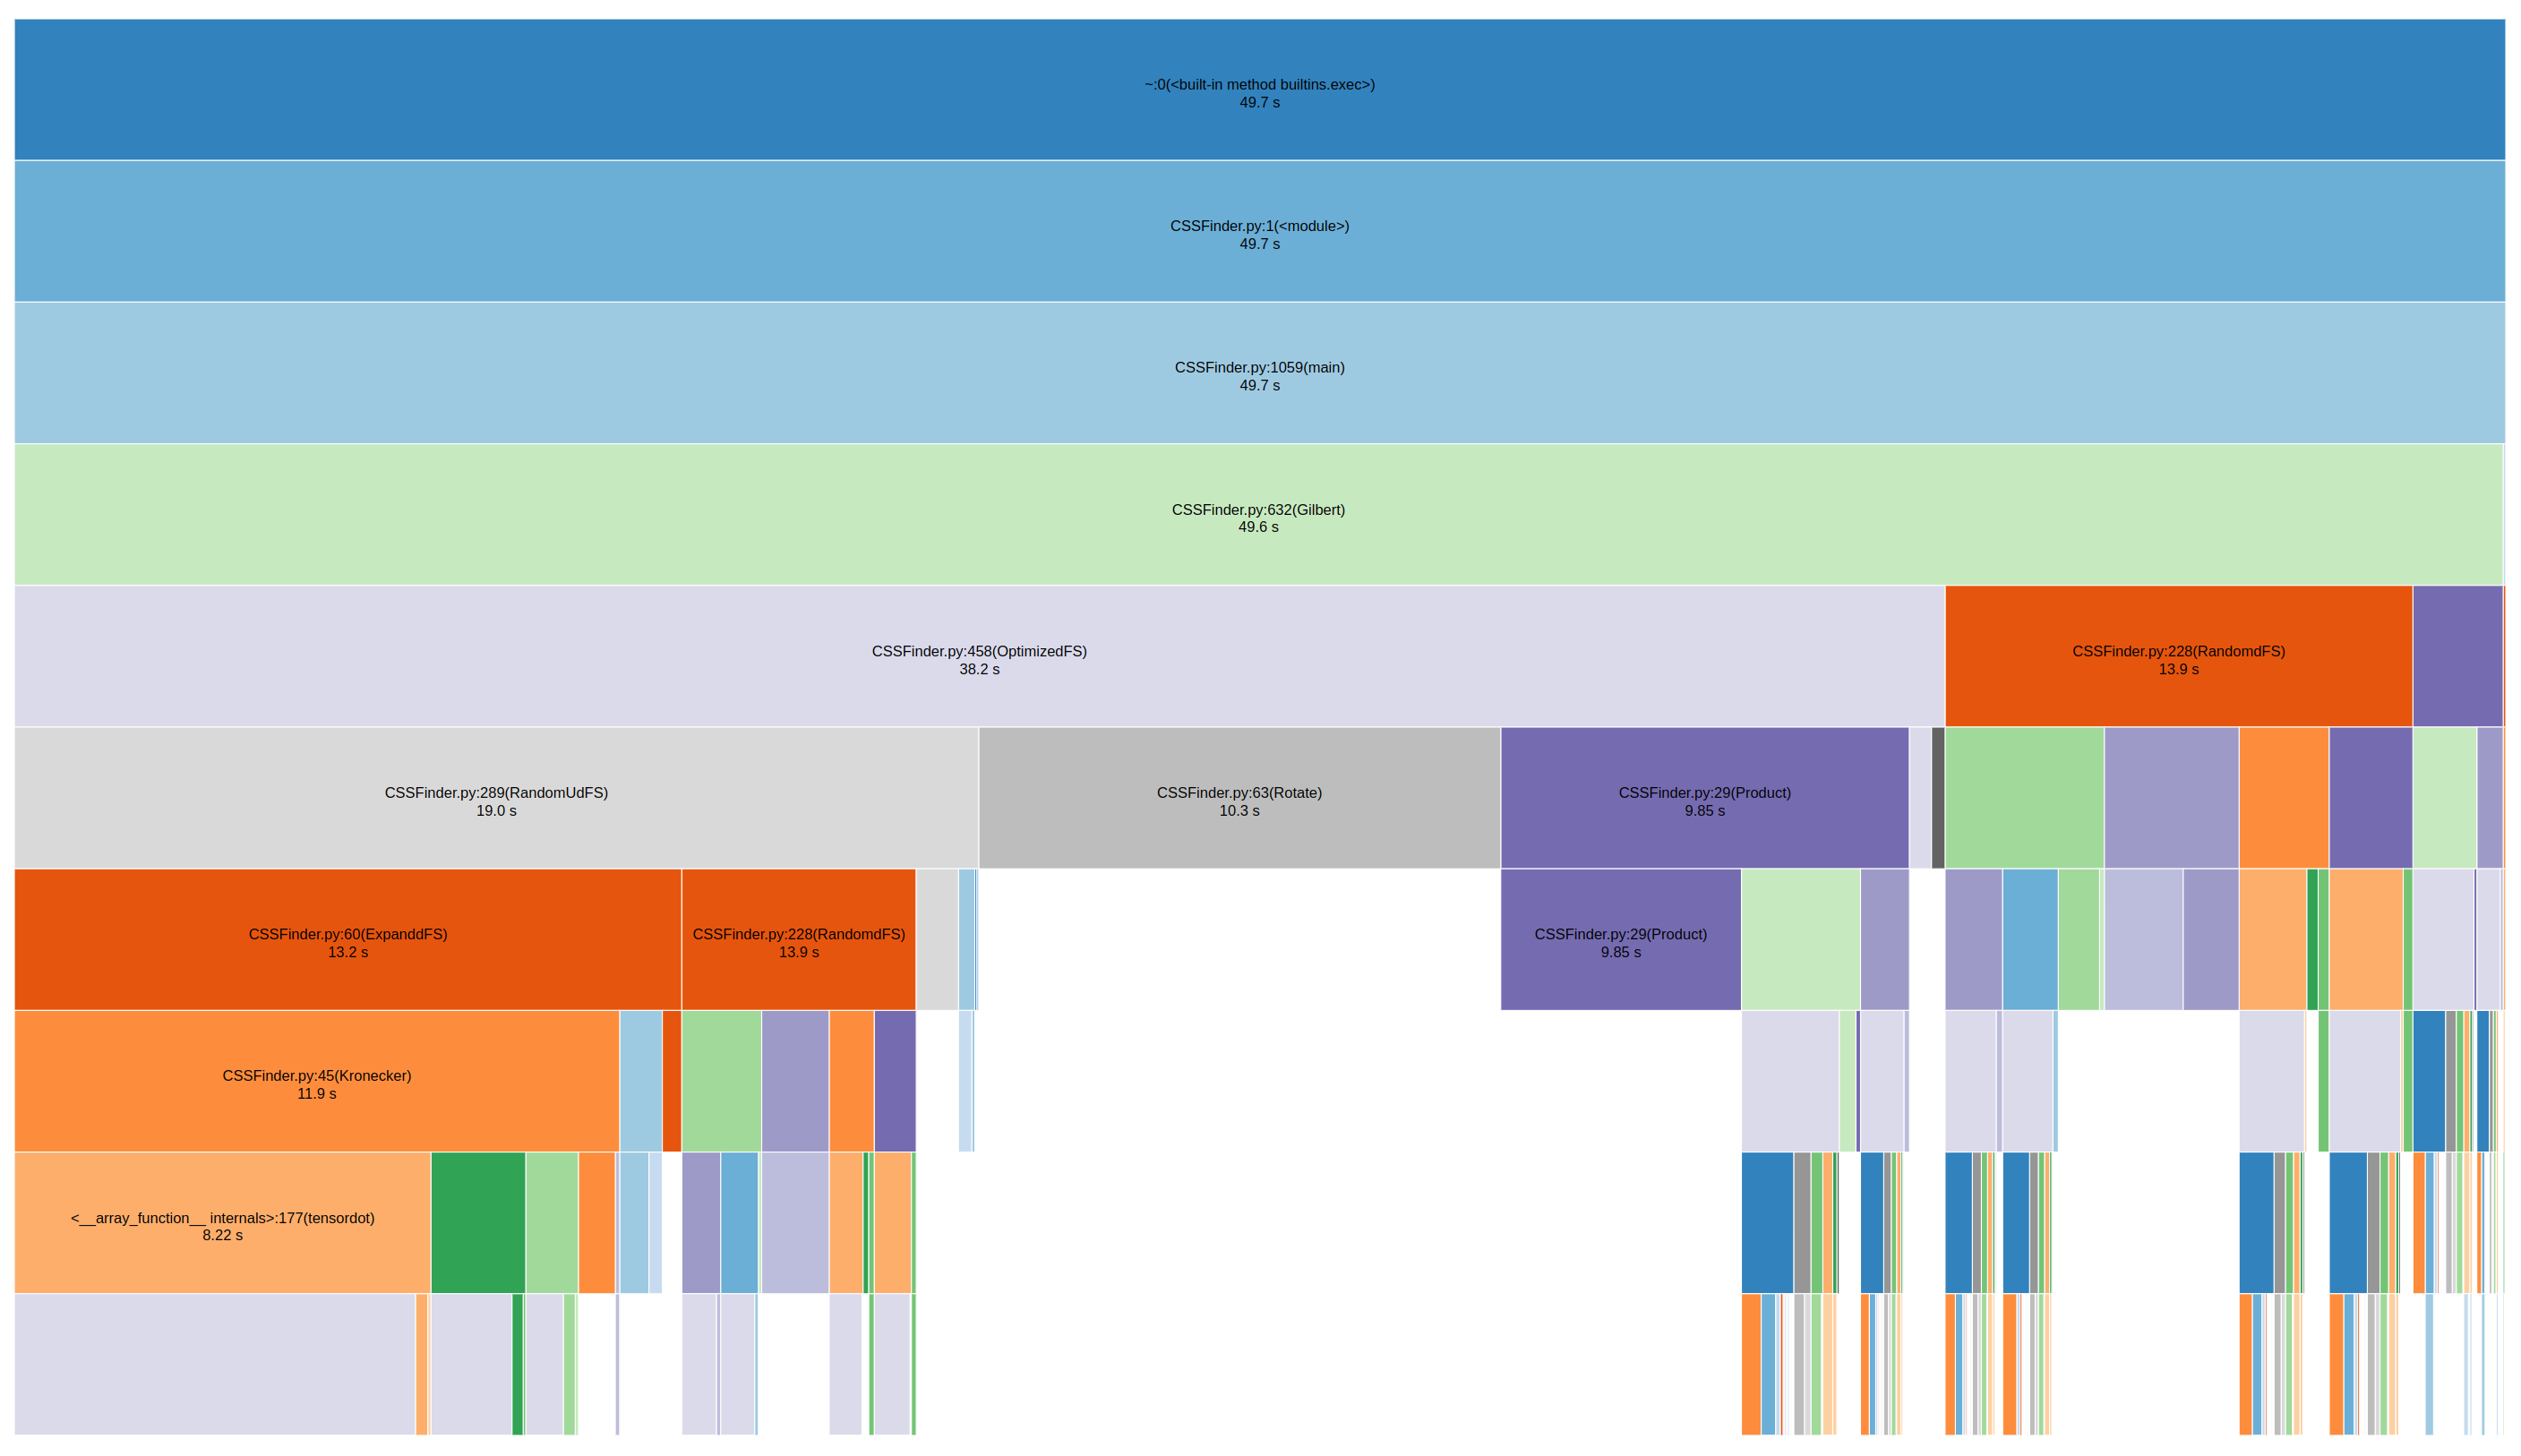
\includegraphics[width=1.0\textwidth]{"resources/profiling_1/graph.png"}
      \caption{Diagram przedstawiający udział całkowitego czasu wykonywania wywołań funkcji w całkowitym czasie programu. Pierwszy blok od góry to pierwsze wywołanie pochodzące z interpretera. Następnie bloki, których opisy zaczynają się od \code{CSSFinder.py} to wywołania w kodzie programu. Najniższe bloki to wywołania do funkcji bibliotek, głównie NumPy. \code{Snakeviz} automatycznie podejmuje decyzję o nie adnotowaniu bloku gdy opis nie ma szansy zmieścić się w obrębie bloku. Program pracował w trybie 1 (full separability of an n-quDit state) na 5 qubitach (macierz $3
      2\times32$ podwójnej precyzji zmiennoprzecinkowych liczb zespolonych)}
    \end{figure}
    \FloatBarrier
    \begin{table}[!ht]
      \tiny
      \centering
      \begin{tabular}{llllll}
  ncalls  & tottime   & percall   & cumtime   & percall   & filename:lineno(function)         \\
  \midrule\midrule
  1       & 1.431e-05 & 1.431e-05 & 49.72     & 49.72     & CSSFinder.py:1(\&lt;module\&gt;)  \\
  1       & 7.526e-05 & 7.526e-05 & 49.68     & 49.68     & CSSFinder.py:1059(main)           \\
  1       & 0.3098    & 0.3098    & 49.63     & 49.63     & CSSFinder.py:632(Gilbert)         \\
  1028    & 0.5381    & 0.0005234 & 38.2      & 0.03716   & CSSFinder.py:458(OptimizedFS)     \\\midrule
  411200  & 0.8332    & 2.026e-06 & 19.03     & 4.627e-05 & CSSFinder.py:289(RandomUdFS)      \\
  595516  & 0.67      & 1.125e-06 & 13.88     & 2.331e-05 & CSSFinder.py:228(RandomdFS)       \\
  411200  & 0.384     & 9.338e-07 & 13.17     & 3.203e-05 & CSSFinder.py:60(ExpanddFS)        \\
  822400  & 0.7256    & 8.823e-07 & 11.94     & 1.452e-05 & CSSFinder.py:45(Kronecker)        \\\midrule
  849257  & 10.3      & 1.213e-05 & 10.3      & 1.213e-05 & CSSFinder.py:63(Rotate)           \\
  1068026 & 6.535     & 6.118e-06 & 9.85      & 9.223e-06 & CSSFinder.py:29(Product)          \\
  1332780 & 2.17      & 1.628e-06 & 4.502     & 3.378e-06 & CSSFinder.py:21(Normalize)        \\
  1332780 & 2.247     & 1.686e-06 & 3.802     & 2.853e-06 & CSSFinder.py:33(Generate)         \\\midrule
  737264  & 0.4225    & 5.73e-07  & 2.548     & 3.456e-06 & CSSFinder.py:18(Outer)            \\
  595516  & 0.4642    & 7.794e-07 & 2.361     & 3.964e-06 & CSSFinder.py:26(Project)          \\
  1233601 & 0.8998    & 7.294e-07 & 1.165     & 9.447e-07 & CSSFinder.py:39(IdMatrix)         \\
  1       & 3.046e-06 & 3.046e-06 & 0.05277   & 0.05277   & CSSFinder.py:96(readmtx)          \\\midrule
  1       & 1.752e-06 & 1.752e-06 & 0.05277   & 0.05277   & CSSFinder.py:552(Initrho0)        \\
  1       & 4.597e-06 & 4.597e-06 & 0.002477  & 0.002477  & CSSFinder.py:1049(DisplayLogo)    \\
  1       & 5.189e-06 & 5.189e-06 & 0.0004394 & 0.0004394 & CSSFinder.py:954(DetectDim0)      \\
  1       & 1.628e-05 & 1.628e-05 & 2.526e-05 & 2.526e-05 & CSSFinder.py:556(Initrho1)        \\\midrule
  1       & 1.903e-06 & 1.903e-06 & 5.671e-06 & 5.671e-06 & CSSFinder.py:599(DefineSym)       \\
  40      & 3.038e-06 & 7.595e-08 & 3.038e-06 & 7.595e-08 & CSSFinder.py:192(writemtx)        \\
  1       & 1.102e-06 & 1.102e-06 & 2.846e-06 & 2.846e-06 & CSSFinder.py:624(DefineProj)      \\
  2       & 2.3e-07   & 1.15e-07  & 2.3e-07   & 1.15e-07  & CSSFinder.py:845(makeshortreport) \\\midrule
\end{tabular}
      \caption{{} Dane dotyczące pracy oryginalnej implementacji programu CSSFinder uzyskane przy pomocy programy cProfile. Ujęte zostały tylko wywołania funkcji z kodu programu CSSFinder. Program pracował w trybie 1 (full separability of an n-quDit state) na 5 qubitach (macierz $3
      2\times32$ podwójnej precyzji zmiennoprzecinkowych liczb zespolonych). Tabela posiada oryginalne nazwy kolumn, nadane przez program \code{snakeviz}. Znaczenia kolumn, kolejno od lewej: \code{ncalls} - ilość wywołań funkcji. \code{tottime} - całkowity czas spędzony w ciele funkcji bez czasu spędzonego w wywołaniach do podfunkcji. \code{percall} - \code{totime} dzielone przez \code{ncalls}. \code{cumtime} - całkowity czas spędzony w wewnątrz funkcji i w wywołaniach podfunkcji. \code{percall} - \code{cumtime} dzielone przez \code{ncalls}. \code{filename:lineno(function)} - Plik, linia i nazwa funkcji.}
    \end{table}
    \FloatBarrier

    Z uzyskanych danych wynika że znakomitą większość (77\%\footnote{Wartość 77\% jak i
    wartości procentowe dalszej części tego akapitu zostały zaokrąglone do jedności, ze względu
    na małe znaczenie rzeczowe części ułamkowych.}) czasu pracy programu zajmuje funkcja
    \code{OptimizedFS()} . W jej wnętrzu 38\% czasu pochłania proces generowania
    losowych macierzy unitarnych, który w dużej mierze wykorzystuje mnożenia tensorowe (26\%).
    Poza funkcją \code{OptimizedFS()}, znaczący wpływ na czas wykonywania ma też funkcja
    `rotate()`, która pochłania około 21\% czasu działania programu. Kolejne 20\% czasu zajmuje
    funkcja \code{product()}, obliczająca odległość Hilberta-Schmidta pomiędzy dwoma stanami.
    Pozostałe wywołania mają stosunkowo marginalny wpływ na czas pracy i ich analiza na
    tym etapie nie niesie za sobą znaczących korzyści.

    Takie wyniki wskazują jednoznacznie że kluczowa dla wydajności jest tu
    maksymalizacja wydajności operacji macierzowych. W uzyskanych danych nie widać problemów
    z operacjami I/O\footnote{I/O - operacje wejścia wyjścia, w tym wypadku odczyt z i pisanie
    do plików.}.

    \subsection{Współbieżność}


    Algorytm z którego korzysta program CSSFinder nie pozwala się efektywnie uwspółbieżniać
    obliczeń dla pojedynczego stanu. O ile możliwe jest współbieżne wykonywanie mnożeń
    macierzowych, to rozsądniejszym rozwiazaniem jest polegać na bibliotekach zewnętrznych,
    jako że są one efektem starań wielu zespołów doświadczonych programistów. Szczególnie
    interesujące są biblioteki które posiadają dedykowane dla platformy, optymalizowane,
    warianty implementacji mnożeń macierzowych i podobnych operacji. Do takich bibliotek
    należy OpenBLAS, wykorzystywany przez NumPy.

    NumPy automatycznie wykorzystuje wiele wątków do mnożeń macierzowych jeśli te są wykonywane
    na odpowiednio dużych macierzach. W przypadku małych macierzy, kosztowność synchronizacji
    obliczeń wielowątkowych przekroczyła uzyskiwane korzyści, szczególnie biorąc pod
    uwagę, że współczesne procesory obsługują instrukcje SIMD, pozwalające na
    uzyskiwanie wysokiej przepustowości obliczeniowej.

    Wykonalne jest uzyskanie współbieżności na poziomie wielu stanów. Ten efekt można całkiem
    efektywnie uzyskać przy pomocy odpowiednio spreparowanych skryptów powłoki,
    wywołujących program wielokrotnie w tle. Jednocześnie wygodniejsze jest posiadanie wbudowanego
    mechanizmu zarządzania zadaniami wbudowanego w program. Z tego względu do nowo
    powstałego kodu dodałem mechanizm automatycznego zarządzania wieloma procesami. Załącza
    się on automatycznie i jest całkowicie niewidoczny dla użytkownika.

    % TODO
    %%  PLOT OF SCRIPT VS SCHEDULER

    %Algorytm jest ściśle sekwencyjny. W nielicznych miejscach gdzie
    % współbieżność można teoretycznie zaimplementować, albo jest już ona zaimplementowana,
    % jak w przypadku mnożeń macierzowych, albo nie daje efektów ze względu na czas który
    % pochłania komunikacja pomiędzy wątkami w języku Python w porównaniu do ilości
    % operacji które można wykonać jednocześnie. Można natomiast efektywnie zaimplementować
    % współbieżność na poziomie wielu zadań. Program może automatycznie zarządzać wieloma
    % procesami które powadzą optymalizację.

    \subsection{Modularyzacja}


    Podczas procesu optymalizacji planowałem wypróbować liczne rozwiązania, które
    wymagały zasadniczych zmian w algorytmie. Jednocześnie część programu odpowiadająca za
    interakcję z użytkownikiem i ładowanie zasobów pozostawała taka sama. Zdecydowałem
    więc że tworzony przeze mnie kod musi być modularny. Tak też program został podzielony
    na część, główną (core) oraz część implementującą algorytm (backend). Korpus jest w całości
    napisany w języku Python i wykorzystuje wbudowany w ten język mechanizm importowania
    w celu wykrywania i ładowania implementacji algorytmu. Dane Macierzowe w obrębie
    korpusu przechowywane są jako obiekty \code{ndarray} z biblioteki NumPy, ze względu
    na uniwersalność w świecie bibliotek do obliczeń tensorowych. Pozwala to na proste podmiany
    implementacji o dowolnie różnym pochodzeniu, co było kluczowe w procesie weryfikacji
    wydajności różnych implementacji.

    \subsection{Dostępne narzędzia}


    \subsubsection{Kompilacja AOT}


    % \footnote{AOT compilation (Ahead Of Time compilation) - kompilacja przed czasem
    % wykonywania programu.}

    Obecnie najpowszechniej używana implementacja języka Python, CPython, posiada możliwość
    korzystania z bibliotek współdzielonych (\code{.so} - Linux, \code{.dll}/\code{.pyd}
    - Windows). Dostęp do funkcji zawartych w takich bibliotekach można uzyskać na kilka
    sposobów:

    \begin{enumerate}
      \item Przy pomocy API modułu \code{ctypes}\cite{Python_ctypes} które pozwala opisać
        interfejs funkcji obcej (tj. takiej która została napisana w języku niższego poziomu
        i skompilowana do kodu maszynowego) i wywołać tak opisaną funkcję.

      \item Poprzez zawarcie w bibliotece odpowiednio nazwanych symboli, automatycznie
        rozpoznawanych przez interpreter języka Python. Takie biblioteki określa się mianem
        modułów rozszerzeń \cite{Extending_Python_With_C_Cpp}. W tym przypadku warto
        dodać, że pomimo, że oficjalna dokumentacja wspomina tylko o językach \code{C} i
        \code{C++}, natomiast powstały biblioteki które pozwalają wykorzystać w łatwy sposób
        wiele innych języków programowania, takich jak \code{Rust} przy pomocy \code{Py03}\cite{PyO3}
        lub \code{GO} z użyciem biblioteki \code{gopy}\cite{gopy}.

      \item Wykorzystując bibliotekę \code{Cython}\cite{Cython_Org}\cite{Cython_The_Best_Of_Both}.
        Oferuje ona dedykowany język, o tej samej nazwie, który jest nadzbiorem języka Python,
        który rozszerza jego składnię o możliwość statycznego typowania. Biblioteka zawiera
        zawieraja transpilator, zdolny przetłumaczyć dedykowany język na C/C++, a następnie,
        wykorzystując osobno zainstalowany kompilator, skompilować do kodu maszynowego.
        % Cython nie wymaga aby w kompilowanym kodzie znajdowały się dodatkowe adnotacje, wzwiązku
        % z czym możliwe jest skompilowanie czystego, nietypowanego, kodu Pythona do kodu maszynowego.
        % Pozwala to na pozbycie się obciążenia ze strony procesu interpretacji oraz
        % skorzystać z optymalizacji, oferowanych przez współczesne kompilatory. Nie usuwa
        % to jednak obciążenia ze strony dynamicznego systemu typów, czyniąc kompilację bez
        % adnotacji mało efektywną.


      \item Kompilując kod pythona z użyciem biblioteki\code{mypyc}\cite{mypyc}. Ta,
        podobnie do Cythona, również zawiera transpilator, natomiast zamiast korzystać z
        dedykowanego języka , bazuje on na dodanych w Pythonie 3.5\cite{Python_3_5} (PEP
        484\cite{PEP_484} i PEP 483\cite{PEP_483}), adnotacjach typów. Jest on rozwijany
        obok projektu mypy - pakietu do statycznej analizy typów dla języka Python,
        również opartej na adnotacjach typów\cite{mypy}.
    \end{enumerate}

    Ponieważ w każdym z wymienionych przypadków, kod niższego poziomu jest kompilowany
    przed dostarczeniem do użytkownika, pozwala to na wykorzystanie zaawansowanych możliwości
    automatycznej optymalizacji dostarczanych przez współczesne kompilatory, na przykład
    LLVM, które jest sercem implementacji \code{clang} (język C++) oraz \code{rustc} (język
    Rust). Wiele bibliotek korzysta z mieszanek wymienionych powyżej metod.

    Powyższe rozwiązania są wykorzystywane przez:
    \begin{itemize}
      \item NumPy

      \item CuPy

      \item Tensorflow

      \item PyTorch
    \end{itemize}

    Każda z tych bibliotek oferuje zestaw funkcjonalności wystarczający do akceleracji
    interesującego nas algorytmu.

    \subsubsection{Kompilacja JIT}


    W momencie pisania tej pracy istnieją dwa szeroko dostępne i aktywnie utrzymywane
    narzędzia oferujące kompilację JIT dla języka Python. Jednym z nich jest pełna alternatywna
    implementacja języka Python - PyPy\cite{PyPy_Home_Page}. Wykonywana przez nią kompilacja
    JIT działa on na podobnej zasadzie do uprzednio wymienionych - śledzi cały kod który
    wykonuje i automatycznie decyduje które fragmenty skompilować do kodu maszynowego\cite{PyPy_JIT}.
    Drugim narzędziem jest biblioteka Numba\cite{Numba_Article}\cite{Numba_Doc}. Ona, w przeciwieństwie
    do PyPy, wymaga aby fragmenty kodu, które mają być skompilowane, miały postać
    funkcji oznaczonych dedykowanymi dekoratorami\footnote{Obecnie dostępny jest też dekorator
    pozwalający na kompilację klas, niestety jest on niestabilny i nie radzi sobie w
    wielu sytuacjach.}.

    \subsection{Optymalizacja}


    Weryfikacja każdej dostępnych metod byłaby czasochłonna oraz często nieuzasadniona -
    wiele z tych narzędzi nie było tworzonych z myślą o przypadku który rozważamy lub
    wykazuje się mniejszą wydajnością od rozwiązań równoważnych. Ostatecznie analizie poddałem
    następujące warianty implementacji programu CSSFinder:

    \begin{itemize}
      \item w języku Python, bazującą na bibliotece NumPy,

      \item w języku Python, bazującą na bibliotece NumPy z kompilacją JIT z użyciem
        pakietu Numba,

      \item w języku Python, bazującą na bibliotece NumPy z kompilacją AOT z
        wykorzystaniem pakiety Cython i kompilatora GCC,

      \item w języku Rust, bazującą na bibliotece ndarray z kompilacją AOT z
        wykorzystaniem rustc (LLVM)
    \end{itemize}

    \subsection{Re-implementacje}


    \subsubsection{ Python i NumPy }


    \subsubsection{ Python i NumPy z JIT }


    \subsubsection{ Python i NumPy z AOT }


    \subsubsection{ Rust }


    \subsection{Precyzja obliczeń}


    Oryginalny program posługiwał się liczbami zespolonymi stworzonymi na bazie
    zmiennoprzecinkowych podwójnej precyzji. Jednak ponieważ analizowane dane utrzymują zakres
    wartości blisko 0, do efektywnych obliczeń nie jest konieczna podwójna precyzja. Podstawową
    zaletą tej zmiany jest zmniejszenie rozmiaru macierzy w pamięci, a to w pozwala na
    umieszczenie większej części macierzy w pamięci podręcznej procesora. Dodatkowo zwiększa
    to przepustowość wektoryzowanego kodu (Zestawy instrukcji FMA uzywają rejestrów o
    rozmiarach 128 i 256 bit, można więc w jednym takim rejestrze umieścić dwukrotnie więcej
    32 bitowych liczb pojedynczej precyzji niż 64 bitowych podwójnej).

    \subsection{Pomiary czasu pracy}


    \subsection{Ponowne profilowanie}


    \subsection{Funkcja kronecker}


    \subsection{Funkcja product}


    \section{Wyniki}


    \section{Dyskusja}
  \end{sloppypar}
  \newpage
  \begin{sloppypar}
    \medskip


    \printbibliography
    [heading=bibintoc, title={Odwołania}]
  \end{sloppypar}
\end{document}